\section{The Meaning of Necessity}
\label{s:semantics}

 
In this section we define our \Nec specification language.  We first
define an underlying programming language, \Loo (\S \ref{sub:Loo}).
We then define an assertion language, \SpecO, which can talk about the
contents of the state, as well as about provenance, permission and
control (\S \ref{sub:SpecO}).  Finally, we define the syntax and
semantics of \susan[]{our full language for writing} \Nec
specifications (\S \ref{s:holistic-guarantees}).


\subsection{\Loo}
\label{sub:Loo} 
%\jm[TODO: mention the type system and the restriction on external method calls]{}
%% We introduce a simple object-oriented language, \Loo, upon 
%% which our specification language sits.
 \Loo is a formal model of an unsurprising, imperative, sequential, 
class based, typed, object-oriented language.
%\susan[Java fields are package private not class private - are fields so important that we need to say this?]{Fields are private to the class where they are defined.}
\Loo is straightforward:
%Given its simplicity, %  the simplicity of \Loo, we do notdefine it here, instead, 
% we direct the reader to
Appendix \ref{app:loo} contains 
the full definitions.
%%and introduce here only % syntax and operational semantics.
%% the concepts relevant to the
%%treatment of the open world guarantees.
%\jm[]{\Loo fields are private in the way fields in Java are private,
%the privacy is class-wide, i.e. they may only be read or written to by 
%objects of the same class.}
\Loo is based on \LangOO 
\cite{FASE}, with some small variations, as well as 
the addition of a % while \LangOO is untyped, \Loo 
 a simple type system -- more in \ref{types}.
%has type based restrictions on external access to private data.}
%\sophiaPonder[added]{Note that the operational semantics only allows filed
%update if the receiver and the object being updated belong to the same class,
%and only allows method calls 
%
%
A \Loo state $\sigma$ consists of a 
heap $\chi$, and a  {stack $\psi$ which is a sequence of frames}.
A frame $\phi$ consists of
local variable map, and a continuation, \ie a sequence of statements to be executed.
 A statement may assign to variables, create new objects and push them to the heap, 
 \susan[create new objects on the heap]{}
perform field reads and writes on objects,  or
 call methods on those objects. 

%Program 
 Modules are mappings
from class names to class definitions. 
Execution 
%takes place
is in the context of  a module $M$ and   \scd{a state $\sigma$},
%It is % Execution
 \scd{defined} via unsurprising small-step semantics of the form \ \ 
   $M, \sigma \leadsto \sigma'$.
The   top frame's continuation contains the statements to be % currently being 
executed next.
 % chopped, as generic 
 % There are several properties  of \Loo that are important to the central topic of this paper. 
 
As discussed in \S \ref{s:approach}, we are interested in guarantees which hold
\sophiaPonder[need to remind reader of internal/external]{during execution of an internal, 
known, trusted module $M$ when linked together with any
unknown, untrusted, module $M'$.} These guarantees need only hold 
when the external module is executing; \scd{we} are not concerned if they are
temporarily broken by the internal module. Therefore, we are only interested in states where the
executing object (\prg{this}) is an external object. 
To express our focus on external states, we define the  \emph{external states semantics}, of the form 
$\reduction{M'}{M}{\sigma}{\sigma'}$, where $M'$ is the external
module, and $M$ is the internal module, and where we
collapse all internal steps into one single step.

 

\begin{definition}[External States Semantics]
\label{def:pair-reduce}
For  
% If we say "internal module", it is sounds as something makes the module be internal
  modules $M$,  $M'$, and % program
   states $\sigma$, $\sigma'$, 
we say that $\ \ \ \ \ \ \ \ \reduction{M'}{M}{\sigma}{\sigma'}\ \ \ \ \ \ \ \ $ if and only if there exist 
$n\in\mathbb{N}$, \scd{and states $\sigma_0$,...$\sigma_n$}, such that
\begin{itemize}
\item
$\sigma$=$\sigma_1$, and  $\sigma'$=$\sigma_n$,
\item
$M' \circ M, \sigma_i \leadsto \sigma_{i+1}$  \ \ \ for all $i\in [0..n)$,
\item
$\class{\sigma}{\scd{\prg{this}}}, \class{\sigma'}{\scd{\prg{this}}}\in M'$,
\item
$\class{\sigma_i}{\scd{\prg{this}}} \in M$\ \ \ for all $i\in [1..n)$.
\end{itemize} 
\end{definition}
\scd{The function $\class{\sigma}{\_}$ is overloaded:}
  applied to a variable, 
$\class{\sigma}{x}$  looks up the variable $x$ in the top frame of $\sigma$, and returns the 
class of the corresponding object in the  heap of $\sigma$,
\scd{while  applied to an address, $\class{\sigma}{\alpha}$  returns
the class of   the object referred by address $\alpha$ in the heap of $\sigma$.}
 The module linking operator $\circ$, applied to two modules, $M'\circ M$, 
 combines the two modules into one module in the obvious way, provided their
domains are disjoint.
Full details in  Appendix \ref{app:loo}.
\begin{figure}[htb]
\begin{tikzpicture}[->,>=stealth',shorten >=1pt,auto,node distance=9mm,
                    thick,
                    external node/.style={circle,draw,minimum size=7mm,font=\sffamily\Large\bfseries, color=blue, fill = blue, text = black, fill opacity = 0.5},
                    internal node/.style={circle,draw,minimum size=7mm,font=\sffamily\Large\bfseries, color=orange, fill = orange, text = black, fill opacity = 0.5}]
    
	\node[external node] (a) {1};
	\node[internal node] (b) [right = of a] {2};
	\node[external node] (c) [right = of b] {3};
	\node[external node] (d) [right = of c] {4};
	\node[internal node] (e) [right = of d] {5};
	\node[internal node] (f) [right = of e] {6};
	\node[external node] (g) [right = of f] {7};
	\node[internal node] (h) [right = of g] {8};
	\node[external node] (i) [right = of h] {9}; 

	\path[every node/.style={font=\sffamily\small}]
		(a) edge[bend left] node [above] {} (b)
		(b) edge[bend left] node [above] {} (c)
		(c) edge[bend left] node [above] {} (d)
		(d) edge[bend left] node [above] {} (e)
		(e) edge[bend left] node [above] {} (f)
		(f) edge[bend left] node [above] {} (g)
		(g) edge[bend left] node [above] {} (h)
		(h) edge[bend left] node [above] {} (i);
\end{tikzpicture}
\begin{tikzpicture}[->,>=stealth',shorten >=1pt,auto,node distance=9mm,
                    thick,
                    external node/.style={circle,draw,minimum size=7mm,font=\sffamily\Large\bfseries, color=blue, fill = blue, text = black, fill opacity = 0.5},
                    internal node/.style={circle,draw,minimum size=7mm,font=\sffamily\Large\bfseries, color=orange, fill = orange, text = black, fill opacity = 0.2, draw opacity = 0.5}]
    
	\node[external node] (a) {1};
	\node[internal node] (b) [right = of a] {2};
	\node[external node] (c) [right = of b] {3};
	\node[external node] (d) [right = of c] {4};
	\node[internal node] (e) [right = of d] {5};
	\node[internal node] (f) [right = of e] {6};
	\node[external node] (g) [right = of f] {7};
	\node[internal node] (h) [right = of g] {8};
	\node[external node] (i) [right = of h] {9}; 

	\path[every node/.style={font=\sffamily\small}]
		(a) edge[bend left=46] node [above] {} (c)
		(c) edge[bend left=46] node [above] {} (d)
		(d) edge[bend left=46] node [above] {} (g)
		(g) edge[bend left=46] node [above] {} (i);
\end{tikzpicture}
   \caption{External States Semantics
     (Def. \ref{def:pair-reduce}). %
     % 
     (A) $\exec{{\color{hotpink}M'} \circ {\color{lightseagreen}M}}{\sigma_1}{\ldots}\leadsto \sigma_9$\ \ \and \ \ \ 
     (B) $\reduction{{\color{hotpink}M'}}{{\color{lightseagreen}M}}{\sigma_2}{\ldots}\leadsto \sigma_9$
    %  (c) $\reduction{{\color{orange}M'}}{{\color{blue}M}}{\sigma_1}{\ldots}\leadsto \sigma_8$
    }
   \label{fig:VisibleStates}
 \end{figure}
 
Fig. \ref{fig:VisibleStates} inspired by \citeasnoun{FASE} provides a simple graphical description of 
our external states semantics: \scd{(A) is the ``normal'' execution after 
linking two modules into one: \ $M' \circ M, ... \leadsto ...$ whereas (B) is the
 external states execution when $M'$ is external,\   $\reduction{M'}{M}{...}{...}$.}
\sophiaPonder[ALL; please read and check]{
Note that whether a module is external or internal depends on our
perspective -- nothing in a module itself renders it internal or external. For example, in
 $\reduction{M_1}{M_2}{...}{...}$ the external module is $M_1$,
  while in  $\reduction{M_2}{M_1}{...}{...}$  the external module is $M_2$.}

\sophiaPonder[moved to earlier]{We  use} the notation\ \  $\reductions{M'}{M}{\sigma}{\sigma'}$ \ 
to denote
zero or more % reduction 
\scd{steps} starting at state $\sigma$ and ending at state $\sigma'$, in the context of internal module 
$M$ and external module $M'$.
 %Not only are we unconcerned 
%with internal states,  we are also unconcerned with  states which cannot ever arise from execution.
\susan[]{We are not concerned with either internal states nor states that cannot ever arise.}
\sophiaPonder[better connection, avoided repetition, tighten]{\emph{Arising} states are those that  may arise by external states execution
starting at some initial configuration:}



\begin{definition}[Arising  States]
\label{def:arising}
For   modules $M$ and  $M'$, a % program
 state $\sigma$ is 
\scd{called} an \emph{arising} state, formally \ \ \ $\arising{M}{M'}{\sigma}$,\ \ \ 
if and only if there exists some $\sigma_0$ such that $\initial{\sigma_0}$ and
$\reductions{M'}{M}{\sigma_0}{\sigma}$.
\end{definition}

\scd{An \emph{Initial}} state's heap
contains a single object of class \prg{Object}, and
its  stack   consists of a single frame, whose local variable map is a
mapping from \prg{this} to the single object, and whose continuation \scd{is}  any statement.
(See Definitions \ref{def:initial} and \ref{def:arising}).

\subsection{\SpecO}
\label{sub:SpecO}
%\SpecO extends \sophiaPonder[drop: the expressiveness]{}   standard %specification 
%\scd{assertion} languages
%with  forms capturing key concepts of software security:
% \emph{Permission}, \emph{Provenance}, and \emph{Control}.

%%\sophiaPonder[]{We define the syntax and semantics of \SpecO, and introduce the concert
%% of assertion encapsulation, as well as some simple means by which we can establish it.}
% assists construction of proofs.

\SpecO is a subset of the \emph{Chainmail} assertions language, \ie
a basic assertion language extended with
object-capability assertions. 


\subsubsection{Syntax of of \SpecO}
The syntax of \SpecO  % assertions 
is given in
Definition \ref{f:chainmail-syntax}.
% the \SpecO specification language.
An assertion may be an expression,   \scd{a query of the defining class of
  an object}, the usual connectives and quantifiers, along 
with three non-standard assertion forms:
\jm[]{(1) \emph{Permission} and (2) \emph{Provenance}, inspired by the capabilities literature, and
(3) \emph{Control} which allows tighter  characterisation of the cause of effects --  
useful for the specification of large APIs.}
\begin{itemize}
\item
\emph{Permission} ($\access{x}{y}$):  
  $x$ has access to $y$.
\item
{\emph{Provenance}} ($\internal{x}$ and $\external{y}$):   $x$ is internal, and $y$ is external.
\item
\emph{Control} ($\calls{x}{y}{m}{\overline{z}}$): 
$x$ calls method $m$ on object $y$ with arguments $\overline{z}$.
\end{itemize}
\sophiaPonder[swap capitalization]{} 


\begin{definition}
Assertions ($A$) \scd{in}  
\SpecO are defined as follows:

\label{f:chainmail-syntax}
 \[
\begin{syntax}
\syntaxElement{A}{}
		{
		\syntaxline
				{e}
				{e : C}
				{\neg A}
				{A\ \wedge\ A}
				{A\ \vee\ A}
				{\all{x}{A}}
				{\ex{x}{A}}
		\endsyntaxline
		}
		{
		\syntaxline
				{\access{x}{y}}
				{\internal{x}}
				{\external{x}}
%		\endsyntaxline
%		}
%		{
%		\syntaxline
				{\calls{x}{y}{m}{\overline{z}}}
		\endsyntaxline
		}
\endSyntaxElement\\
\end{syntax}
\]

\jm[Def. 3.3 seems to hang here awkwardly ...]{}


\end{definition}



\subsubsection{Semantics of \SpecO}
The semantics of \SpecO  % assertions 
is \scd{given} in Definition \ref{def:chainmail-semantics}. 
% \SpecO makes use of several language features of 
\sophiaPonder[used to say "several" -- is it so?]{}
% \Loo that can be found in Apdx. \ref{app:loo}. Specifically, $\eval{M}{\sigma}{e}{v}$
\scd{We   use the evaluation relation, $\eval{M}{\sigma}{e}{v}$,
which says that the expression $e$ evaluates
to value $v$ in the context of state $\sigma$ and module $M$.
Note} that expressions in \Loo may be recursively defined, and thus evaluation 
\scd{need not always} % may not necessarily 
 terminate. Nevertheless, the logic of $A$ remains classical because recursion is restricted
to expressions, and not generally to assertions.
\sophiaPonder[JULIAN: Do we have such a proof indeed?]{We have taken this approach from \citeasnoun{FASE}, which also contains a mechanized Coq proof that assertions are classical \citeasnoun{coqFASE}.}
\jm[yes. there is a proof. I cited the proof. Is this too much of a ``this is us!'' flag?]{}
%  The full
The semantics of $\hookrightarrow$ are unsurprising (see Fig.\ref{f:evaluation}).

Shorthands:  \susan[what does resp mean? respectively? if so it would read better by deleting it]{}
 $\interpret{\phi}{x} = v$  means that $x$ maps to
value $v$ in the local variable map of frame $\phi$, $\interpret{\sigma}{x} = v$ means that $x$ 
maps to $v$ in the top most frame of $\sigma$'s stack, and $\interpret{\sigma}{x.f} = v$
has the obvious meaning. The terms $\sigma.\prg{stack}$,  
%resp. 
$\sigma.\prg{contn}$, 
%resp. 
$\sigma.\prg{heap}$     mean the stack, 
%resp. 
the continuation at the
top frame of $\sigma$, %resp. 
and the heap of $\sigma$.
The term $\alpha\!\in\!\sigma.\prg{heap}$ means that $\alpha$ is in the domain of the heap of $\sigma$, and \emph{$x$ fresh in $\sigma$} means that 
$x$ isn't in the variable map of the top frame of $\sigma$, 
while the substitution  $\sigma[x \mapsto \alpha]$ is applied to the top frame of $\sigma$.
$C\in M$ means that class $C$ is in the domain of module $M$. 

\begin{definition}[Satisfaction % of \SpecO 
of Assertions \scd{by a module and a state}] 
\label{def:chainmail-semantics}
We define satisfaction of an assertion $A$ by a % program 
state $\sigma$ with \sophiaPonder[used to say "internal" I think this was wrong]{}
 module $M$ as:
\begin{enumerate}
\item
\label{cExpr}
$\satisfiesA{M}{\sigma}{e}$ \ \ \ iff \ \ \  $\eval{M}{\sigma}{e}{\true}$
\item
\label{cClass}
$\satisfiesA{M}{\sigma}{e : C}$ \ \ \ iff \ \ \  $\eval{M}{\sigma}{e}{\alpha}$ \textit{and} $\class{\sigma}{\alpha} = C$
\item
$\satisfiesA{M}{\sigma}{\neg A}$ \ \ \ iff \ \ \  ${M},{\sigma}\nvDash{A}$
\item
$\satisfiesA{M}{\sigma}{A_1\ \wedge\ A_2}$ \ \ \ iff \ \ \  $\satisfiesA{M}{\sigma}{A_1}$ and 
$\satisfiesA{M}{\sigma}{A_2}$
\item
$\satisfiesA{M}{\sigma}{A_1\ \vee\ A_2}$ \ \ \ iff \ \ \  $\satisfiesA{M}{\sigma}{A_1}$ or 
$\satisfiesA{M}{\sigma}{A_2}$
\item
$\satisfiesA{M}{\sigma}{\all{x}{A}}$ \ \ \ iff \ \ \  
$\satisfiesA{M}{\sigma[x \mapsto \alpha]}{A}$, \ 
\ \ \ for some $x$ fresh in $\sigma$, and for all $\alpha\!\in\!\sigma.\prg{heap}$.
\item
$\satisfiesA{M}{\sigma}{\ex{x}{A}}$ \ \ \ iff \ \ \  
$\satisfiesA{M}{\sigma[x \mapsto \alpha]}{A}$, \ 
\ \ for some $x$ fresh in $\sigma$, and for some $ \alpha\!\in\!\sigma.\prg{heap}$. 
\item
\label{cAccess}
$\satisfiesA{M}{\sigma}{\access{x}{y}}$ \ \ \ iff \ \ \  
\begin{enumerate}
\item
\label{c1}
$\interpret{\sigma}{x.f}={\interpret{\sigma}{y}}$ for some $f$, \\
  or
\item
\label{c2}
{$\interpret{\sigma}{x}=\interpret{\phi}{\prg{this}}$}, {and $\interpret{\sigma}{y}=\interpret{\phi}{z}$}\ \ \ \
for some variable $z$, and some frame $\phi$ in $\sigma.
\prg{stack}$.
\end{enumerate}
\item
\label{cInternal}
$\satisfiesA{M}{\sigma}{\internal{x}}$ \ \ \ iff \ \ \  
$\textit{classOf}(\sigma,x) \in M$
\item
\label{cExternal}
$\satisfiesA{M}{\sigma}{\external{x}}$ \ \ \ iff \ \ \  
$\textit{classOf}(\sigma,x) \not\in M$
\item
\label{cCall}
$\satisfiesA{M}{\sigma}{\calls{x}{y}{m}{z_1, \ldots, z_n}}$ \ \ \ iff \ \ \ 
\begin{enumerate}
\item
$\sigma.\prg{contn} = (w := y'.m(z'_1,\ldots,z'_n)\scd{; s})$,\ \ \scd{for some 
variable $w$, and some statement $s$},
\item
$\satisfiesA{M}{\sigma}{x = \prg{this}}$
\ \ and \ \ 
$\satisfiesA{M}{\sigma}{y = y'}$,
\item
$\satisfiesA{M}{\sigma}{z_i = z'_i}$\ \ \ for all $1\!\leq i\!\leq n$
\end{enumerate}
\end{enumerate}
\end{definition}

 
\scd{ The assertion ${\access{x}{y}}$ (defined in  \ref{cAccess})
requires  that $x$ has access to $y$
either through a field of $x$ (case \ref{c1}),
or through some call in the stack, where $x$ is the receiver and $y$ is one of the
arguments (case \ref{c2}).
 The assertion %$\satisfiesA{M}{\sigma}
 ${\calls{x}{y}{m}{z_1, \ldots, z_n}}$  (defined in \ref{cCall}) 
requires that the current receiver (\prg{this}) is $x$, and that it calls the method $m$ on $y$ with
 arguments $z_1$, ... $z_n$.\footnote{It does \emph{not} mean  that somewhere in the 
 call stack there exists a call from $x$ to $y.m(...)$.}
 Note that in most cases, satisfaction of an assertion not only depends on the state $\sigma$, but 
also depends on the module in the case of expressions (\ref{cExpr}), class membership
(\ref{cClass}), and internal or external provenance (\ref{cInternal} and \ref{cExternal}).}


\scd{We now} define what it means for a module to satisfy an assertion:
 $M$ satisfies  $A$ if any state arising from external steps execution of that
module with any other external module  satisfies $A$. 
 
\begin{definition} [Satisfaction % of \SpecO 
of Assertions
\scd{by a module}] 
\label{def:mdl-sat}
For a module $M$ and assertion $A$, we say that\ \  $\satisfies{M}{A}$ \ \ if and only if 
for all modules $M'$, and all $\sigma$, if $\arising{M'}{M}{\sigma}$, then $\satisfiesA{M}{\sigma}{A}$.
\end{definition}

 
\scd{In the current work we assume the existence of a proof system that judges}
$\proves{M}{A}$, to prove  satisfaction of assertions. 
 We will not define such a judgment, but will rely on its existence see Theorem \ref{thm:soundness}).
We define soundness of such a judgment in the usual way:

\begin{definition}[Soundness of \SpecO Provability]
\label{ax:specW-prove-soundness}
A judgment of the form $M \vDash A$ is \emph{sound}, if for all
 modules $M$ and assertions $A$, \ if $\proves{M}{A}$ then $\satisfies{M}{A}$.
\end{definition}

%\subsection{Assertion Encapsulation, Wrapping, and Types}
%\label{s:semantics:encaps}
%
%\subsubsection{Wrapping}
%
%We define a useful shorthand \jm[]{for a critical concept}: the predicate $\wrapped{\prg{o}}$  states 
%that only \internalO objects have access to \prg{o}.
%The object \prg{o} may be either \internalO or \externalO.
%\begin{definition}[Wrapped]
%$\wrapped{o}\ \triangleq\ \all{x}{\neg \access{x}{o}\ \vee\ \internal{x}}$
%\end{definition}
%
%Wrapping is a very useful concept. For example, the balance of an account whose
%  password is wrapped,  will not decrease in the next step.
%  Often, API implementations contain objects whose capabilities, while  crucial for the implementation, if exposed,
%would break the intended guarantees of the API. Such objects need to remain wrapped - c.f.
%such an example in section 5. 
% %Quite often,  o
%% Objects with many capabilities 
%%may be kept wrapped so as to adhere to the API's guarantees. 
% %\susan [I would remove this]{For example, in 
% % Sect \ref{s:examples} the objects of class \prg{Ledger} would allow withdrawals from an account
% % without knowledge of the password; nevertheless \prg{Mod4} adheres to (***) because
% % the \prg{Ledger} objects are always wrapped.}}
%%\jm[@sophia - yes let's keep this]{}
%%Wrapped is critical as it captures the conditions under \jm[]{an interaction
%%with the \internalM module is necessary}. 
%%\jm[]{As an example, consider the Bank Account example from Section \ref{s:outline}: if} only \internalO
%%objects have access to an account's password, then
%%it follows that access to the password may not 
%%be gained except by an interaction with the \internalM
%%module, and subsequently if the \internalM module
%%is secure we know that the password cannot be leaked.
%%\jm[]{This predicate forms a core aspect of Part 2 mentioned in Section \ref{s:outline},
%%and is elaborated on more in Section \ref{s:classical-proof}.}
%
%\subsubsection{Encapsulation} In Sec. \ref{s:outline} we used  encapsulation of \SpecO assertions 
% in our proof of adherence to \Nec specifications.
%We said that   $A$ is encapsulated by  $M$ if it cannot be invalidated unless an
%internal method was called. 
%Here we refine this concept, to allow for ``conditional'' encapsulation:
%$M\ \vDash A\ \Rightarrow\ \encaps{A'}$ expresses that in states which satisfy $A$, the assertion 
%$A'$ cannot be invalidated, unless a method from $M$ was called.
%
%\begin{definition}[Assertion Encapsulation]
%\label{def:encapsulation}
%\sd{An assertion $A'$ is \emph{encapsulated} by module $M$ and assertion $A$, written as}\ \  $M\ \vDash A\ \Rightarrow\ \encaps{A'}$, \ \ if and only if
%for all external modules $M'$, and all states $\sigma$, $\sigma'$
%such that $\arising{M}{M'}{\sigma}$:
%
%\begin{tabular}{lr}
%$\;\;\;\;$- $\reduction{M'}{M}{\sigma}{\sigma'}$  & \rdelim\}{3}{4mm}[$\;\;\;\Rightarrow\;\;\;$  $\exists x,\ \overline{z}. (\ \satisfiesA{M}{\sigma}{\calls{\_}{x}{m}{\overline{z}} \wedge\ \internal{x}}\ )$] \\
%$\;\;\;\;$- $\satisfiesA{M}{\sigma}{A \wedge  A'}$ \\
%$\;\;\;\;$- $\satisfiesA{M}{\sigma' \triangleleft \sigma}{\neg A'}$   
%\end{tabular} 
%\end{definition}
%
%%\susan[I found this confusing. If you omit the highlighted sentence it is easier to understand.]{We use ${\sigma' \triangleleft \sigma}$ for the state as in $\sigma'$ but with the variable bindings as in the top frame from $\sigma$.} 
%We will define 
%${\sigma' \triangleleft \sigma}$ in  Def. \ref{d:adapt}, but 
%we first look at some examples.
%In both \prg{Mod2} and \prg{Mod3} the \prg{balance} of an account cannot change
%unless an internal method was called:
%\\
%\strut \hspace{1cm}
%$\prg{Mod2}\ \vDash \prg{a}:\prg{Account}\ \Rightarrow\ \encaps{\prg{a.balance}=\prg{bal}}$
%\\
%\strut \hspace{1cm}
%$\prg{Mod3}\ \vDash \prg{a}:\prg{Account}\ \Rightarrow\ \encaps{\prg{a.balance}=\prg{bal}}$
%
%%\susan[Does this help the story move on? I would omit it]{
%%Note that encapsulation of an assertion does not imply encapsulation of its negation; 
%%for example $\wrapped{o}$ is encapsulated, but $\neg  \wrapped{o}$ is not.}
%
%
%\subsubsection{Types}
%\label{types}
%
%\sophiaPonder[modified]{To allow for an easy way to judge encapsulation of
%assertions, we assume a very simple type system, where field, method arguments
%and method results are annotated with classes, and the type system checks 
%that field assignments, method calls, and method returns adhere to these expectations.
%Because the type system is so simple, we do not include its specification in the paper.
%Note however, that the type system} has one further implication: modules are typed 
%in isolation, thereby implicitly prohibiting
%method calls from internal objects to external objects. 
%
%\sophiaPonder[]{Based on this type system, we define a predicate $Intrnl(e)$, in Apdx. \ref{s:encap-proof},
%which asserts that any object reads during the evaluation of $e$ are internal.
%Thus, any assertion that only involves $Intrnl(\_)$ expressions is encapsulated, more in Apdx. \ref{s:encap-proof}.}
%
%\sophiaPonder[]{Finally, a further small addition to the type system 
%assists the knowledge that an object is wrapped: Classes may
%be annotated as \enclosed. A \enclosed object  
%cannot be accessed by external objects; that is, it is always wrapped. 
%The type system needs to ensure that objects of \enclosed type
%are never returned from method bodies, this is even simpler than in \cite{confined}. 
%\susan[I would omit this]{Again, we omit the detailed description of this
%simple type system.
%}}


%\jm[]{Finally, \Loo has a simple class based type system where 
%classes may be optionally annotated as \enclosed. An object 
%of an \enclosed type may not be accessed by module-external
%objects. This helps simplify the demonstrative proof of the running 
%Bank Account example (\S\ref{s:examples}). In order to enforce this 
%restriction, methods of non-\enclosed classes are prohibited from
%returning \enclosed objects.}

%\jm[]{The type system is included to allow a simple and convenient way to prove that access to certain 
%objects is restricted. This restriction simplifies the proof of our running example to a manageable degree,
%however it is not fundamental to the definition of either the  \Nec specification language or logic, 
%and could easily be removed.}

 

\subsubsection{Inside}

We define
%%%a useful shorthand \jm[]{for a critical concept}: the
a final shorthand 
predicate $\wrapped{\prg{o}}$ which states 
that only \internalO objects have access to \prg{o}.
The object \prg{o} may be either \internalO or \externalO.
\begin{definition}[Inside]
%%%%%$\wrapped{o}\ \triangleq\ \all{x}{\neg\access{x}{o}\ \vee\ \internal{x}}$
%%%%%
$\wrapped{o}\ \triangleq\ \all{x}{\access{x}{o}\ \Rightarrow\ \internal{x}} $ 
\end{definition}

%\noindent
%(Compare with \citeasnoun{ownalias} where 
%$\access{x}{o} \Rightarrow\ 
%(\prg{x } \texttt{\textcolor{blue}{inside}}~\texttt{\textcolor{blue}{owner}}(\prg{o})).)$

\inside is a very useful concept. For example, the balance of an account whose
  password is \inside  will not decrease in the next step.
  Often, API implementations contain objects whose capabilities, while  crucial for the implementation, if exposed,
would break the intended guarantees of the API. Such objects need to remain \inside - see
such an example in Section \ref{s:examples}. 
 
% \jm[adaptation doesn't fit here. perhaps we move to 3.3? i.e. in the discussion of the \Nec specs?]{}
%\subsubsection{The meaning of adaptation}   
%\sophiaPonder[new]{We introduce the adaptation operation $\adapt {\_} {\_}$ to allow us to
%``see a  state   through the lens of another state''.
%Assume, for example a state $\sigma_0$ which satisfies $A_0$ where $A_0 \triangleq \prg{a}:\prg{Account} \wedge \prg{a.balance}=100$.
%Assume that $\sigma_1$ is the result of executing $\prg{a.transfer(p,10)}$ where \prg{p} is \prg{a}'s password, while $\sigma_2$ is the result of executing $\prg{a=new Account}$. 
%We have that $\satisfiesA {...}{\sigma_0} {A_0}$, and 
%${...},{\sigma_1} \nvDash{A_0}$, and $ {...}{\sigma_2}\nvDash {A_0}$. However, the difference between
%the two executions is that the former modified the object at \prg{a}, and the latter did not; it only modified
%the mapping for variable \prg{a}. Therefore, we want to define an adaptation operator, such that
%${...},{\adapt {\sigma_1} {\sigma_0}} \nvDash{A_0}$ but $\satisfiesA {...}{\adapt {\sigma_2} {\sigma_0}} {A_0}$.}
%
%\sophiaPonder[]{In the definition below, the heap of $\adapt{\sigma'}{\sigma}$ is taken from
%$\sigma'$, and the stack is   mostly taken from $\sigma'$, except that the variable map of the
%top frame consists of the variable map of the top frame of $\sigma$, expanded
%with fresh variables ($\overline{v}$) 
%to correspond to the variables of the top frame of $\sigma'$, and in the continuation the free variables are renamed to $\overline{v}$.}
%
%
%%
%%
%%  These assertions may contain variables, whose denotation might change during
%%program execution: the 
%%map may change, variables may be overwritten, or the entire local variable maps may be lost on a method return.
%%For this reason, before we provide the semantics of our \Nec specification language, we first introduce an adaptation operator
%%to account for variable renaming throughout the execution of a program.
%\begin{definition}
%\label{d:adapt}
%$\adapt{\sigma'}{\sigma} \triangleq (\chi', \{\prg{local} := \beta[\overline{v} \mapsto \beta\scd{'}(\overline{z}')], \prg{contn}:= [\overline{z'}/\overline{v}]c'\} : \psi)$
%where 
%\begin{itemize}
%\item
%$\sigma = (\_, \{\prg{local}:=\beta; \prg{contn}:=\_\} : \_)$, and
%$\sigma' = (\chi', \{\prg{local}:=\beta', \prg{contn}:=c'\} : \psi)$
%\item
%$dom(\beta') = \overline{z'}$, $dom(\beta) \cap \overline{v} = \emptyset$, and $|\overline{z'}| = |\overline{v}|$
%\end{itemize}
%\end{definition}

%\jm[]{Def. \ref{d:adapt} allows satisfaction to take variable renaming during evaluation into account. 
%As an example, consider the following code snippet.}
%\begin{lstlisting}[frame=lines]
%x.f := y
%x := z
%\end{lstlisting}
%\jm[]{After the evaluation of line 1 , \texttt{x} has access to \texttt{y}, however when we overwrite \texttt{x} in line 2, 
%this is no longer necessarily true, as \texttt{x} might now refer to a different object, even though the object previously referred to 
%by \texttt{x} has not changed. A similar issue might occur when either calling a method, or returning from a method, as 
%the entire variable map changes under such circumstances. Adaptation (Def. \ref{d:adapt}) provides a convenient way to refer to 
%objects across time, while ignoring rewrites and new frames.}




\subsection {\Nec Specifications}
\label{s:holistic-guarantees}

Our \Nec specification language extends \SpecO with novel 
 \emph{necessity operators}.
In this section we define its syntax (Definition \ref{f:holistic-syntax}) and semantics 
(Definition \ref{def:necessity-semantics}).
We have the following three operators:
 



\begin{description}
\item[Only If]
[$\onlyIf{A_1}{A_2}{A}$]: If an arising % program
  state satisfies $A_1$, and after some execution, a state % program 
 satisfying $A_2$ is reached, 
then the original  
state must have also satisfied $A$.
 \sophiaPonder[chopped]{}
 %e.g. if the balance of a bank account changes over time, then there must be some external object in the current 
%program  state that has access to the account's password.
% \paragraph{Single-Step Only If}
\item[Single-Step Only If]
[$\onlyIfSingle{A_1}{A_2}{A}$]: If an arising %program
  state satisfies $A_1$, and after a single step of execution, a state satisfying $A_2$ is reached, 
then the original %program 
state must have also satisfied $A$.
\sophiaPonder[chopped]{}
%e.g. if the balance of a bank account changes over a single execution step, then that execution step must be a method call to the bank \prg{transfer} method.

%\paragraph{Only Through}
\item[Only Through]
[$\onlyThrough{A_1}{A_2}{A}$]: If an arising %program 
 state satisfies $A_1$, and after some execution, a state satisfying $A_2$ is reached, then  execution must have passed through some \jm[]{\emph{intermediate}} state satisfying $A$ 
\sophiaPonder[chopped]{}
% e.g. if the balance of an account changes over time, then the bank's \prg{transfer} method must have been called 
% in some intermediate state. Note 
--  the   \emph{intermediate} \jm[]{state} % state where $A$ is true
satisfying $A$ might be the \emph{starting}  
or the \emph{final} state.
\end{description} 

%\begin{figure}[t]
\begin{definition}[\Nec Syntax] The syntax of
\Nec  Specifications ($S$)
% in   \Chainmail   
is as follows:
% \footnotesize

\footnotesize
\[
\begin{syntax}
\syntaxElement{S}{}
		{
		\syntaxline
				{A}
				{\onlyIf{A_1}{A_2}{A_3}}
				{\onlyThrough{A_1}{A_2}{A_3}}
		\endsyntaxline
		}
		{
		\syntaxline
				{\onlyIfSingle{A_1}{A_2}{A_3}}
		\endsyntaxline
		}
\endSyntaxElement\\
\end{syntax}
\]
%\caption{Syntax of \Chainmail Necessity Specifications}
\label{f:holistic-syntax}
\end{definition}
%\end{figure}
\normalsize



\jm[]{\paragraph{Relationship between \Nec Operators}
The three \Nec operators defined in Def. \ref{f:holistic-syntax}
can be related by generality. An \emph{Only If} ($\onlyIf{A_1}{A_2}{A}$) implies
a \emph{Single-Step Only If} ($\onlyIfSingle{A_1}{A_2}{A}$), since if $A$ is 
a necessary precondition for multiple steps, then it must be a necessary 
precondition for a single step. \emph{Only If} also implies 
an \emph{Only Through}, where the intermediate state is the starting state
of the execution. }
%This relationship can be better observed when we 
%encode the \Nec operators with traditional temporal operators:
%\jm[]{\begin{description}
%\item[Only If:] $\onlyIf{A_1}{A_2}{A}\ \equiv\ A_1\ \wedge\ \Diamond A_2\ \longrightarrow\ A$
%\item[Single-Step Only If:] $\onlyIfSingle{A_1}{A_2}{A}\ \equiv\ A_1\ \wedge\ \bigcirc A_2\ \longrightarrow\ A$
%\item[Only Through:] $\onlyThrough{A_1}{A_2}{A}\ \equiv\ (A_1\ \longrightarrow\ (\Diamond (A\ \wedge\ \Diamond A_2) \vee \neg \Diamond A_2))$
%\end{description}
%}

\subsection{SD's proposal for motivation of adaptation}

In order to give semantics to the three necessity operators, we will need an auxiliary, renaming operator 
$\adapt{}{}$ for states, where
 $\adapt{\sigma'}{\sigma}$ maps the variables in the top frame of a state $\sigma'$ according to the variables in 
 ${\sigma}$.

Here is why this operator is needed: A naive, first approach to defining the semantics of 
$\onlyIf{A_1}{A_2}{A}$, would have a roughly the following form:\footnote{roughly, as we omitted mentioning the module}  
\[ (*) \ \ \ \  \sigma \models \onlyIf{A_1}{A_2}{A}\ \ \ \ \mbox{iff} \ \ \ \ \forall \sigma'.[\ \sigma \models {A_1} \wedge \sigma' \models {A_2} \wedge \sigma \leadsto^* \sigma' \ \rightarrow  \sigma \models A \ ] \]

The problem with  the definition (*), is that it does not take into account that the variable bindings in $\sigma'$ might be different to those in $\sigma$. For example, assume  we had a module  which defined accounts with immutable owners. Then, in the for such a module, we would expect that for all $\sigma$:
\[ (**)\ \ \ \ \sigma \models \onlyIf{\prg{a:Account} \wedge \prg{o}\neq\prg{null} \wedge \prg{a.owner}={\prg{o}}}{ \prg{a.owner}\neq{\prg{o}}}{\prg{false}} \]

Namely, (**) asserts that once initialized, the value of the field \prg{owner} becomes immutable. \footnote{There exists no state $\sigma$, where the value $\prg{a.owner}$ is not \prg{null}, and might change at some point in the future.} However, if we apply the definition from (*), then (**) does \emph{not} hold. As a counterexample, assume a state $\sigma_1$ where   $\sigma_1 \models \prg{o}\neq \prg{null} \wedge \prg{a.owner}=\prg{o}$, and $\sigma_1$'s continuation is \prg{o:=new Object}.  By executing the continuation, we obtain a $\sigma_2$, where $\sigma_1 \leadsto  \sigma_2$ and where $\sigma_2  \models \prg{a.owner}\neq{\prg{o}}$. The latter holds, because the value of \prg{o} is different in $\sigma_1$ and $\sigma_2$. 

This is why we introduced the  renaming operator $\adapt{\sigma'}{\sigma}$  which modifies $\sigma'$ slightly, so the frame of $\sigma$ and $\sigma'$ are identical.  With such an operator, we refine   (*) as follows
\[ (***)\  \ \ \  \sigma \models \onlyIf{A_1}{A_2}{A}\ \ \ \ \mbox{iff} \ \ \ \ \forall \sigma'.[\ \sigma \models {A_1} \wedge \adapt{\sigma}{\sigma'}  \models {A_2} \wedge \sigma \leadsto^* \sigma' \ \rightarrow  \sigma \models A \ ] \]

It remains to define the operator $adapt$ ...

 
\noindent
\textbf{end of SD proposal}

\kjx{
\subsubsection{Adaptation: viewing the future through the lens of the past.}
%
%
Consider a specification that says for an account's balance to go down
from 100 to 50, a \prg{transfer} method must be called on that account:}
%% \onlyThrough{$\prg{a}:\prg{Account} \wedge \prg{a.balance}=100$}
%%   {$\prg{a.balance}=50$}
%%   {$\calls{\_}{a}{transfer}{\_,\_}$}
%
%%NecessityBankSpec  $\triangleq$
%
\begin{lstlisting}[language = Chainmail, mathescape=true, frame=lines]
                    from a:Account $\wedge$ a.balance == 100
                        to a.balance == 50
                        onlyThrough $\calls{\_}{\prg{a}}{\prg{transfer}}{\_,\_}$
\end{lstlisting}
%
%
%
%
\kjx{
This specifications refers to three different program states: at
the start when the balance is 100; and the end when it's 50; and
somewhere between when \prg{transfer} is called.  For this
specification to make sense, the bindings of variables like \prg{a}
must refer to the same object in each state, in particular, bindings
over the future states must refer to the same object as in the past
state. (Because \Loo's objects' classes, types, or fields never change
and are never deleted from the heap, we can at least be sure any
object that exists in some state will still exist in all arising future
states).
}

\kjx{
%potential for variable name clashes between different program states.
  We deal with this via an \emph{adaptation} operator \cite{FASE}. We
  write
  $\adapt {\sigma'} {\sigma}$
  to view a future state $\sigma'$ from the perspective of a current
  (or past) state $\sigma$. 
%  
%  To deal with this we introduce the adaptation operation $\adapt {\_}
%  {\_}$ to allow us to
%  
%``see a  state   through the lens of another state''.
%Assume, for example a state $\sigma_0$ which satisfies $A_0$ where
%$A_0 \triangleq \prg{a}:\prg{Account} \wedge \prg{a.balance}=100$. 
%% Assume that $\sigma_1$ is the result of executing $\prg{a.transfer(p,10)}$ where \prg{p} is \prg{a}'s password, while $\sigma_2$ is the result of executing $\prg{a=new Account}$. 
%% We have that $\satisfiesA {...}{\sigma_0} {A_0}$, and 
%% ${...},{\sigma_1} \nvDash{A_0}$, and $ {...}{\sigma_2}\nvDash {A_0}$. However, the difference between
%% the two executions is that the former modified the object at \prg{a}, and the latter did not; it only modified
%% the mapping for variable \prg{a}. Therefore, we want to define an adaptation operator, such that
%% ${...},{\adapt {\sigma_1} {\sigma_0}} \nvDash{A_0}$ but $\satisfiesA {...}{\adapt {\sigma_2} {\sigma_0}} {A_0}$.
%
%
%
Def.\ref{d:adapt} shows how $\adapt{\sigma'}{\sigma}$ constructs a new
state, taking the heap and most of the stack from the future state 
$\sigma'$. We replace the top frame's variable map 
with the variable map from the top frame of the past state $\sigma$,
avoiding name clashes by renaming the 
variables in the top frame of $\sigma'$ with fresh variables
($\overline{v}$) and renaming free variables in the continuation similarly.
}

%
%
%  These assertions may contain variables, whose denotation might change during
%program execution: the 
%map may change, variables may be overwritten, or the entire local variable maps may be lost on a method return.
%For this reason, before we provide the semantics of our \Nec specification language, we first introduce an adaptation operator
%to account for variable renaming throughout the execution of a program.
%\begin{definition}
%$\adapt{\sigma'}{\sigma} \triangleq (\chi', \{\prg{local} := \beta[\overline{v} \mapsto \beta\scd{'}(\overline{z}')], \prg{contn}:= [\overline{z'}/\overline{v}]c'\} : \psi)$
%where 
%\begin{itemize}
%\item
%$\sigma = (\_, \{\prg{local}:=\beta; \prg{contn}:=\_\} : \_)$, and
%$\sigma' = (\chi', \{\prg{local}:=\beta', \prg{contn}:=c'\} : \psi)$
%\item
%$dom(\beta') = \overline{z'}$, $dom(\beta) \cap \overline{v} = \emptyset$, and $|\overline{z'}| = |\overline{v}|$
%\end{itemize}
%\end{definition}

\begin{definition}
\label{d:adapt}
$\adapt{\sigma'}{\sigma} \triangleq (\chi', \phi'' : \psi')$
where 
\begin{itemize}
\item
$\sigma = (\chi, \phi : \psi)$ 
and
$\sigma' = (\chi', \phi' : \psi')$
\item
$\phi = \{\prg{local}:=\beta; \prg{contn}:=\_\}$, and
$\phi' = \{\prg{local}:=\beta', \prg{contn}:=c'\}$
\item
$\phi'' = \{\prg{local}:=\beta[\overline{y} \mapsto rng(\beta')]; \prg{contn}:=[\overline{y}/dom(\beta')]c'\}$
\item
$\overline{y}$ is fresh $\beta$ and $\beta'$, and $|\overline{y}| = |dom(\beta')|$
\end{itemize}
\end{definition}

\begin{figure}[htb]
\newcommand{\mathsmall}[1]{\substack{\scalebox{0.8}{$#1$}}}
\begin{figure}[tbp]
\begin{tabular}{clclc}
 \begin{minipage}{0.27\textwidth}
 $\sigma:$\\
% ~ \\
 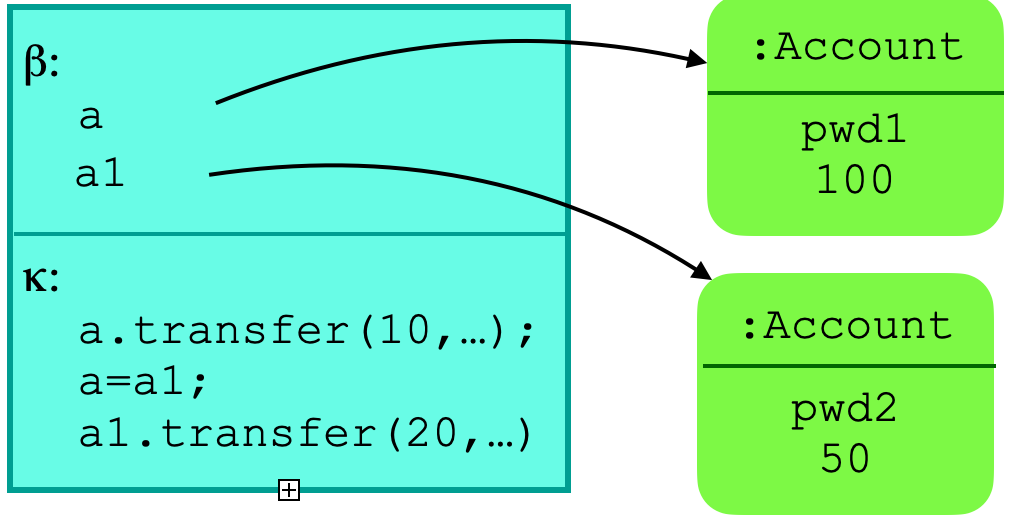
\includegraphics[width=\linewidth]{diagrams/adapt1.png}
   \end{minipage}
 & \ \ \ &
 \begin{minipage}{0.27\textwidth}
  $\sigma':$\\
 % ~ \ \\
  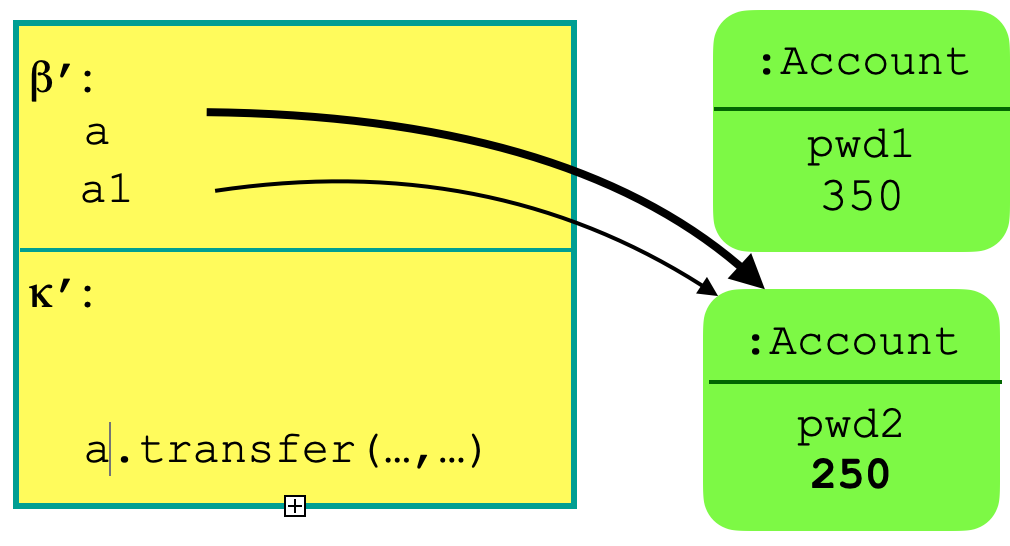
\includegraphics[width=\linewidth]{diagrams/adapt2.png}
   \end{minipage}
   & \ \ \  &
    \begin{minipage}{0.27\textwidth}
$\adapt {\sigma'}{\sigma}:$\\
% ~ \\
  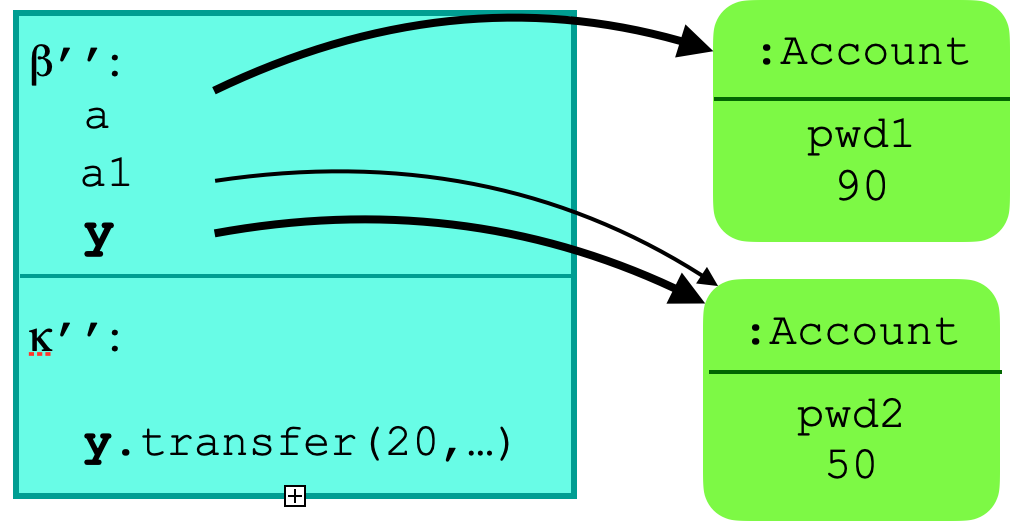
\includegraphics[width=\linewidth]{diagrams/adapt3.png}
   \end{minipage}
\end{tabular}

%\begin{tikzpicture}[->,>=to,shorten >=1pt,auto,node distance=5.5mm,
%                    thick,
%                    state/.style={circle,draw,minimum size=7mm,font=\sffamily\bfseries, color=hotpink, fill = hotpink, text = black, fill opacity = 0.5, scale=0.9},
%                    dots/.style={
%                    minimum size=7mm,
%                    font=\sffamily\Large\bfseries, 
%                    color=lightseagreen, 
%                    text = black, 
%                    fill opacity = 0.5},
%                    space/.style={
%                    minimum size=7mm,
%                    font=\sffamily\Large\bfseries, 
%                    color=lightseagreen, 
%                    text = black, 
%                    fill opacity = 0.5},
%                    arrow/.style={
%                    minimum size=7mm,
%                    font=\sffamily\Large\bfseries, 
%                    color=lightseagreen, 
%                    text = black, 
%                    fill opacity = 0.5},
%                    models/.style={
%                    minimum size=7mm,
%                    font=\sffamily\Large\bfseries, 
%                    color=lightseagreen, 
%                    text = black, 
%                    fill opacity = 0.5},
%                    decoration = snake]
%    
%    \node[space] (s) at (0,0) {};
%	\node[state, label={270:$\mathsmall{\vDash A_1}$}] (a) at (3.85,0) {$\sigma_1$};
%%	\node[space] (b) [right = of a] {};
%	\node[state, label={270:{$\mathsmall{\vDash A_2}$}}] (c) [right = of a] {$\sigma_n$};
%	\draw [decorate, ->]
%	(a) -- (c);
%\end{tikzpicture}
\caption{Illustrating adaptation
}
\label{fig:Adaptation}
\end{figure}

   \caption{Example of the adaptation operator
     (Def. \ref{d:adapt}). %
     Note: in $\sigma$, $\sigma'$, and $\adapt{\sigma'}{\sigma}$, all but the top frame of the stack is elided for simplicity.
    }
   \label{fig:adaptation}
 \end{figure}
 
\jm[]{Adaptation may seem complex, however it is esentially a variable renaming operator. Fig. \ref{fig:adaptation} provides an example 
where the assertion $\access{\prg{this}}{\prg{set}}$
is invalidated by only the method call \prg{set.add(x)}, even though the object graph remains the same. This invalidation does not
reflect a meaningful change to what any object has access to, and in order to preserve the intention of the assertion, the $\triangleleft$ operator
appropriately rewrites $\sigma'$ to maintain the variable names of $\sigma$.}

\subsubsection{Semantics of \Nec Specifications}


We   now define  semantics of specifications,  $M \vDash S$, 
%the semantics of the Necessity Specifications,
%  in Definition \ref{def:necessity-semantics}.  The definition goes 
by cases over the four possible syntactic forms: 


\noindent
\begin{definition}[\Nec Semantics]
\label{def:necessity-semantics}
For any assertions   $A_1$, $A_2$, and $A$,  we define \\


$\bullet$ \ $\satisfies{M}{{A}}$ \ \ \ iff\ \ \ for all $M'$, $\sigma$,\ if $\arising{M}{M'}{\sigma}$, then $\satisfiesA{M}{\sigma}{A}$. (see Def. \ref{def:mdl-sat})\\

%$\bullet$ \ $\satisfies{M}{{A}}$ \ \ \ as defined in \ref{def:mdl-sat} \\

$\bullet$ \ $\satisfies{M}{\onlyIf {A_1}{A_2}{A}}$ \ \ iff\ \  for all $M'$, $\sigma$, $\sigma'$, such that $\arising{M'}{M}{\sigma}$; \\ % and\\

\begin{tabular}{lr}
$\;\;\;\;$- $\satisfiesA{M}{\sigma}{A_1}$  & \rdelim\}{3}{3mm}[$\;\;\;\Rightarrow\;\;\;$  $\satisfiesA{M}{\sigma}{A}$] \\
$\;\;\;\;$- $\satisfiesA{M}{\sigma' \triangleleft \sigma}{A_2}$   \\
$\;\;\;\;$- $\reductions{M'}{M}{\sigma}{\sigma'}$   \\
\end{tabular}\\ 

$\bullet$ \  $\satisfies{M}{\onlyIfSingle {A_1}{A_2}{A}}$\ \ iff\ \   for all $M'$, $\sigma$,   $\sigma'$, such that $\arising{M}{M'}{\sigma}$: \\

\begin{tabular}{lr}
$\;\;\;\;$- $\satisfiesA{M}{\sigma}{A_1}$  & \rdelim\}{3}{3mm}[$\;\;\;\Rightarrow\;\;\;$  $\satisfiesA{M}{\sigma}{A}$] \\
$\;\;\;\;$- $\satisfiesA{M}{\sigma' \triangleleft \sigma}{A_2}$   \\
$\;\;\;\;$- $\reduction{M'}{M}{\sigma}{\sigma'}$   \\
\end{tabular}\\ 
  
$\bullet$ \  $\satisfies{M}{\onlyThrough {A_1}{A_2}{A}}$ \ \ iff\ \  for all $M'$, $\sigma_1$,   $\sigma_n$, such that $\arising{M}{M'}{\sigma_1}$: \\

\begin{tabular}{lr}
$\;\;\;\;$- $\satisfiesA{M}{\sigma_1}{A_1}$  & 
\rdelim\}{3}{3mm}%[\makecell{Some really \\ longer text}]
[$\;\;\;\Rightarrow\;\;\;$\pbox{9cm}{$\forall \sigma_2, \ldots, \sigma_{n-1}$.  \\ 
(\ \ $\forall i\!\in\![1..n).\ \reduction{M'}{M}{\sigma_i}{\sigma_{i+1}}$   \ $\Rightarrow$
$\exists i\!\in\![1..n]. \  \satisfiesA{M}{\sigma_i \triangleleft \sigma_1}{A}$ \ \ )   }] \\
$\;\;\;\;$- $\satisfiesA{M}{\sigma_n\triangleleft \sigma}{A_2}$   \\
$\;\;\;\;$- $\reductions{M'}{M}{\sigma}{\sigma_n}$   \\
\end{tabular} 
\end{definition} 


\sophiaPonder[chopped]{}
%We are now able to state what the necessary preconditions to critical functions in 
%software are, including safety properties of software in the open world. The semantics
%of \emph{Single-Step Only If} allow for the statement of such necessary preconditions
%for any execution step for any program to achieve a certain outcome. The semantics
%of \emph{Only If} and \emph{Only Through} allow us to raise these necessary preconditions
%to any arbitrary number of execution steps, and thus allow for reasoning about 
%the execution of an entire program.
% 



%SD chopped below; find it too "generic"
% Both of these specifications are important, and are both used as intermediate steps
%when we present the full proof of \prg{NecessityBankSpec} later in Section \ref{s:examples}.
%\Nec thus provides us with a rich language for talking about the necessary conditions
%under which critical actions within of our software are allowed to occur. 


%\jm[]{It is worth discussing the semantics of \Nec specifications and their 
%relation to typical logical consequence and Hoare logic. A classical Hoare triple, 
%$\hoare{P}{C}{Q}$, denotes that any program state that satisfies $P$, after execution 
%of program $C$, will result in a program state that satisfies $Q$. Thus, $P$ represents 
%a subset of program states that after execution of $C$ results in a program state satisfying $Q$.
%Conversely, $Q$ represents a superset of program states resulting from the execution of $C$ in 
%a program state satisfying $P$. Thus, we can soundly strengthen the left hand side ($P$), and weaken
%the right hand side ($Q$). This intuition extends to all three specifications. 
%For example, from \prg{NecessityBankSpec'}, while it is somewhat contrived, we are able to
%strengthen the ``left hand side'' by adding information, and weaken the ``right hand side'', 
%and conclude that}
%\begin{lstlisting}[language = Chainmail, mathescape=true, frame=lines]
%NecessityBankSpec'''  $\triangleq$  from a:Account $\wedge$ a.balance == bal $\wedge$ bal == x + y $\wedge$ y > 0
%                       nxt a.balance == x
%                       onlyIf $\exists$ o.[$\external{\texttt{o}}$ $\wedge$ $\access{\prg{o}}{\prg{a}}$]
%\end{lstlisting}
%\jm[]{This follows because in the above specification, (a)\prg{x < bal}, and thus \prg{a.balance = x} implies and $a.balance < bal$,
%and (b) if an object calls a method on another object, it follows that it has access to that object.
%More generally, given a Single-Step Only-If specification, 
%$\onlyIfSingle{A_1}{A_2}{A}$, $A_1$ and $A_2$ represent a subset of single step execution paths starting from a program state 
%satisfying $A_1$ and reaching a program state satisfying $A_2$, that have $A$ as a necessary precondition. 
%In the same way the converse is true, i.e. $A$ represents a superset of initial program states
%for execution starting at a state satisfying $A_1$ and reaching a state satisfying $A_2$ after a single step of execution.
%As with Hoare logic, we are able to soundly strengthen the left hand side ($A_1$ and $A_2$)
%and strengthen the right hand side ($A$). This intuition also extends to Only-If and Only-Through specifications. 
%In some places later in this paper, we use the distinction ``\emph{left hand side}'' of a \Nec specification
%to denote the two left most assertions in the specification, and ``\emph{right hand side}'' to denote
%the necessity precondition.}
 
 
